\chapter{Introduction} % Main chapter title
\graphicspath{ {/Users/kaksonenlab/Desktop/figures/} }
\label{Ch:Intro} % Change X to a consecutive number; for referencing this chapter elsewhere, use \ref{ChapterX}

\section{Endocytosis and cell trafficking pathways}
The plasma membrane serves as the defining barrier between the internal and external cell, thus creating cellular identity, and facilitating evolution out of the primordial soup into a defined structure that can regulate entry of signals into the cell. In eukaryotes, and with increasing complexity, in multicellular eukaryotes, tuning cellular response to external signals has resulted in a complex network of signaling pathways, and tight coupling of these pathways with the process of endocytosis. Endocytosis is defined as the uptake of molecules too big to pass through the plasma membrane. It involves the invagination of the plasma membrane into a cargo-filled tube, and culminates in the severing of this tube to form a cargo-filled vesicle, whose components and contents are then targeted to other cellular organelles for either degradation or recycling. 

\begin{figure}[H]
	\centering
	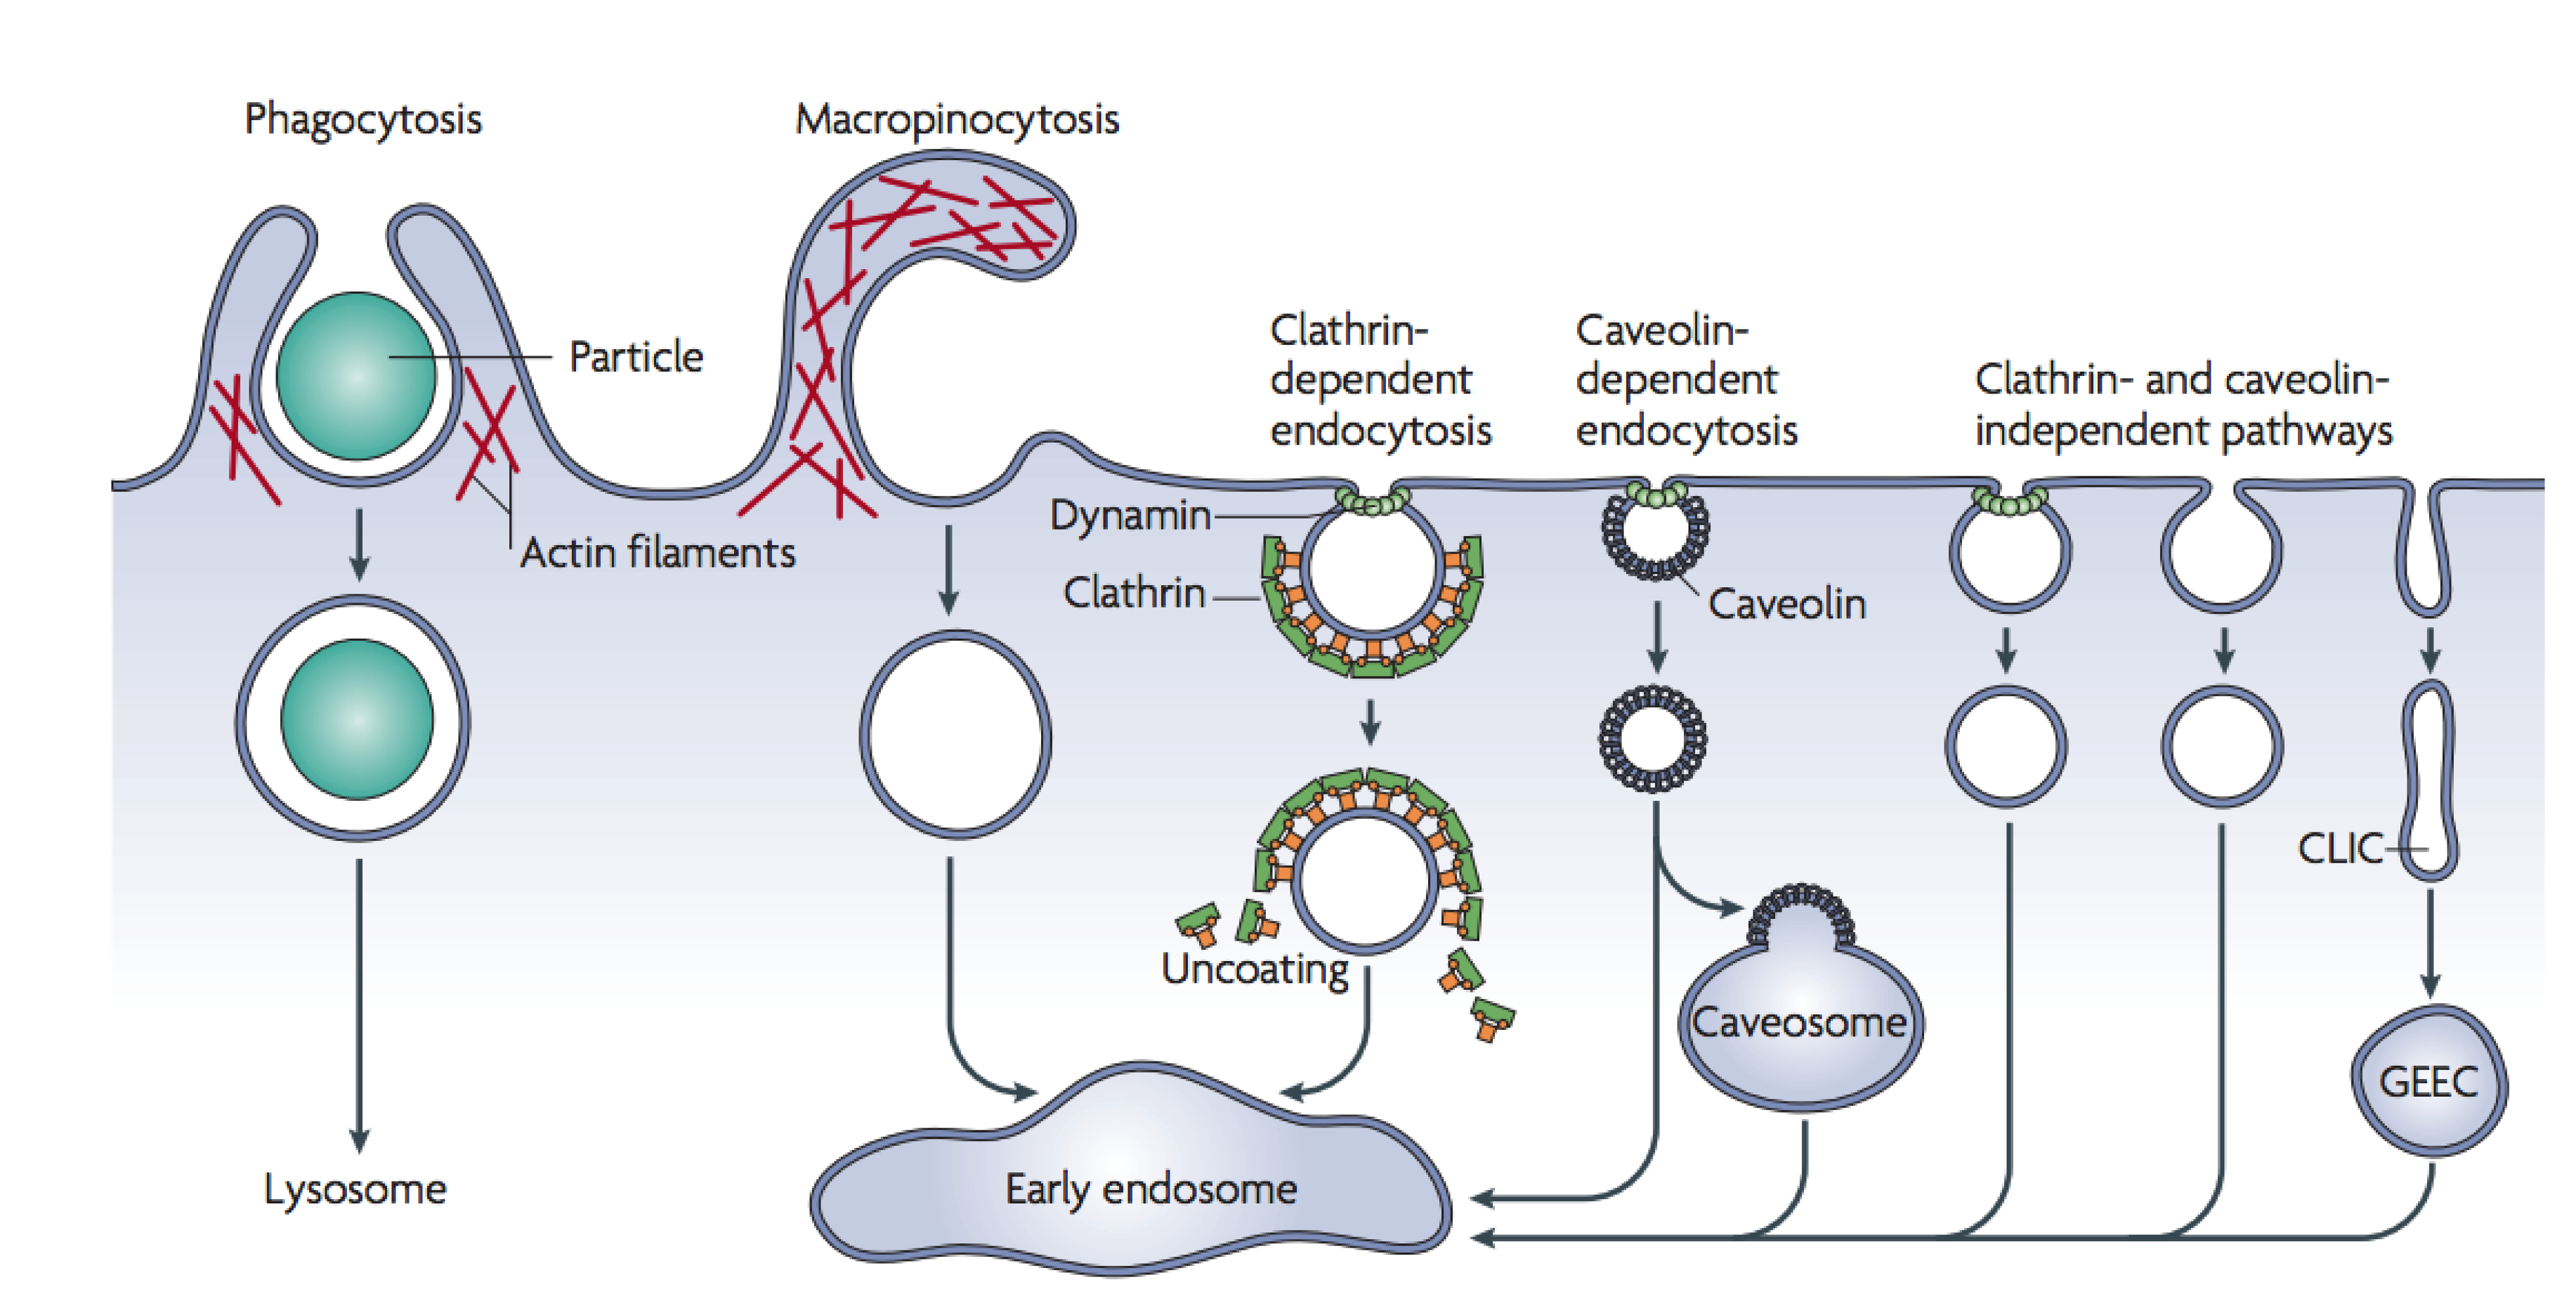
\includegraphics[scale=0.3]{figures/intro/Fig1_mayor}
	\caption[Endocytic pathways in cells]
	{Some of the endocytic pathways in mammalian cells. Large particles are incorporated by phagocytosis, bulk fluid by macropinocytosis. A large array of cargo is taken into the cell via CME and calveolin-dependent endocytosis. Vesicles formed by these pathways are targeted to the early endosome. Clathrin and calveolin-independent pathways incorporate cargo and involve different geometries, including tubular "clathrin- and dynamin-independent carriers" (CLIC), that arrive at "GPI-anchored protein enriched early endosomes" (GEEC), before they are transported to endosomes.  \textit{Reprinted by permission from Springer Nature: Nature Reviews Molecular Cell Biology (Mayor and Pagano, 2007), copyright (2007)}}
\end{figure}


Apart from internalizing cargo, endocytosis allows regulation of the plasma membrane itself: its lipid and protein composition, and therefore many physical and biochemical properties like tension, rigidity, surface-receptor composition and localization. Cargo taken up by endocytic pathways include these surface-receptors and their ligands, that are transported across the cell, taking part in a signaling cascade, and forming the link between cell signaling and endocytosis.


\vspace{5mm}
Somewhat dramatically, endocytosis “constitutes the major communications infrastructure of the cell. As such, it governs almost all aspects of the relationships of the cell with the extracellular environment and of intracellular communication. Its evolution constitutes, arguably, the major driving force in the evolution of prokaryotic to eukaryotic organisms”1.  Plasma membrane regulation and internalization of signaling molecules are critical for the function of the cell. Among the vast array of important cargo that are taken up via endocytosis are cholesterol2,3, insulin4, and other hormones. Not surprisingly, many human diseases have been linked to defects in the endocytic pathway like familial hypercholesterolemia2,3 -the study of which established the field of endocytosis-, Alzheimer’s5, and some types of cancer6. The importance of the endocytic machinery as the entry portal of the cell is evident in the fact that it is hijacked by pathogens like viruses and bacteria to enter host cells7. Other components of the cellular signaling pathway transmit signals across the cell and between various organelles like the Golgi apparatus and endoplasmic reticulum. These membranes undergo similar transitions of the bounding membrane, and have mechanistic and biochemical similarities8,9. 




Although many early discoveries relating to endocytic pathways were identified in mammalian cell types10,11, description of endocytosis in S.cerevisiae12 marked the beginning of important findings that were made in the yeast and later verified in mammalian cells. The ease of genetic manipulation, availability of the completed sequence of the yeast genome, and relative simplicity of endocytic pathways- there is only one- drove several discoveries that established yeast as a powerful model organism13,14.



\section{Clathrin-mediated endocytosis}
Many different endocytic pathways that facilitate the internalization of cargo at the plasma membrane exist, as depicted in Fig.2, all differing in the size and type of cargo. Of them, Clathrin-mediated endocytosis (CME), is universal among eukaryotes and contributes to 90\% of cargo trafficked into the cell15. First identified by studying yolk uptake in mosquitos, ultrastructural studies of their oocytes (where the concentration of uptake events is high enough to be easily studied) identified a bristly coat formation on the cell membrane and similarly bristly vesicles, that then lost this coat and fused to eventually form yolk bodies in the mature oocyte16. The bristle was noted in several cell types, and was later identified as a lattice of a single highly conserved protein17. This protein was named Clathrin, derived from the latin word for lattice. Clathrin is formed of light and heavy chains incorporated into a triskelion18 that assembles into closed hexagonal and pentagonal structures on the inner leaflet of the plasma membrane. Clathrin-mediated endocytosis has, since four decades ago, been recognized has an ubiquitous mechanism of membrane uptake in cell types ranging from the frog presynaptic membrane19 to rat vas deferens20. 

\vspace{5mm}
Clathrin and associated proteins do not only interact with the plasma membrane. It has also been observed localizing to the trans-golgi network (TGN); these clathrin-coated vesicles mediate traffic from the TGN to the endosome. Specification of vesicle target to different cellular compartments is achieved by Clathrin interaction with specialized adaptor proteins like the adaptor protein complexs (AP), which specify Golgi-to-early endosome traffic, while Golgi-localized gamma-adaptin (GGA) complexes specify Golgi-to-late endosome traffic. These membrane associations, among others form components of the cellular signaling pathway that transmit signals across the cell and between various organelles like the Golgi apparatus and endoplasmic reticulum. These membranes undergo similar transitions of the bounding membrane, and have some mechanistic and biochemical similarities13,14. 




	
\section{CME in mammalian and yeast cells }
		\subsection{Clathrin is required for mammalian CME}
		That the clathrin lattice is responsible for remodeling the plasma membrane and selecting cargo was speculated in the first papers that noted the “bristly” coat16,21.  In multicellular organisms like C.elegans, clathrin depleted by RNAi results in decreased endocytic uptake in oocytes and dead progeny22, in D.melanogaster, deletion of clathrin heavy chain results in embryonic lethality23. In Hela cells, knock-down of the heavy chain by RNAi results in decrease in endocytosis by 80\%24; essentially, endocytosis fails in the absence of clathrin. The exact contribution of clathrin in the progression of endocytosis has been heavily debated, but its involvement itself has not. Although several genes involved in CME in yeast were found to be homologues of the mammalian machinery, however, early work in yeast revealed that clathrin is not necessary for endocytosis25. Loss of clathrin changes the size of the vesicles formed at scission, and leads to decrease in the number of established endocytic sites26,27: it appears to affect establishment of sites and regulation of scission. It became apparent that though the mammalian and yeast systems were mechanistically similar and most of the yeast endocytic proteins had mammalian homologues28, there are some significant differences.


		\subsection{Actin forces are required for yeast CME}
		Cortical actin patches were first seen in S.cerevisae, that were later established as endocytic sites from the colocolization of other endocytic proteins. While the mammalian CME uptake is heavily dependent on clathrin, the yeast system relies on actin and its proper organization for endocytosis29. Not only is actin itself necessary for the intiation of plasma membrane deformation30, coupling the endocytic coat to actin are necessary for internalization31,32.  The cell wall surrounding the plasma membrane in yeast cells induces a high intracellular turgor pressure33, which could explain the high force requirement for membrane deformation in yeast. 


	
		\subsection{CME in yeast is highly regular}
		In yeast, over fifty proteins are recruited, interact, and disassembly during this process. In mammals as well as in yeast, the proteins that arrive at an endocytic site can be distributed into different modules according to their relative time of recruitment and function. A variable initiation phase assembles coat proteins on the plasma membrane and establishes an endocytic site. While the later proteins show relatively high variability in both recruitment as well as time spent at sites in mammalian cells, in yeast this initiation is followed by a very stereotypic sequence of events that assembles coat proteins, nucleates actin, organizes the actin network, invaginates a membrane tube, and finally severs the membrane to produce cargo-filled vesicles26. Coat proteins arrive upon initiation of endocytic sites, the actin and WASP modules arrive next, and includes actin nucleating proteins, actin, actin-binding proteins that organize the actin network and produce forces that begin to pull the membrane into the cytoplasm. The scission module arrives last, and regulates the final shape transitions of the endocytic site from tubular membrane to vesicle. 

		\vspace{5mm}
		Sterotypicity of the post-initiation stages of yeast endocytosis has allowed averaging the behavior of various proteins from multiple endocytic events. Tracking and averaging the behavior of these proteins has led to understanding the spatial and temporal regulation of endocytosis in remarkable detail26,34,35. The multiple stages of endocytosis are discussed below. 
		
 


			\subsubsection{Early initiation phase}
			A variable initiation phase establishes endocytic sites and selects cargo36. The earliest proteins to arrive at sites, Ede1 and Syp1 are not required to form endocytic sites. Deletion of an entire seven protein set of early endocytic proteins (Ede1, Syp1, Yap1801/1802, Apl1, Pal1, Pal2) does not prevent endocytosis. It seems that the initiation of endocytosis in yeast is independent of the recruitment of any one protein, and is likely a result of several different cooperative or independent factors36, that could give the process robustness in the absence of alternate pathways for uptake of essential nutrients and signals. The variability in this phase could also provide a “check-point”, to ensure that sufficient cargo is loaded28 before later (energy consuming) phases are triggered. 

			
			\subsubsection{Coat module}
			Coat proteins serve to template later proteins35, as well as form the link between the actin module32, ingressing membrane, and cargo associated with it. Unlike in mammalian cells, as mentioned earlier, clathrin adaptors and the clathrin triskeleon are not necessary for the progression of sites, although deletion of clathrin introduces a high variability in the timing of scission27. 
			
			\vspace{5mm}
			Deletion of coat proteins Sla2 and Ent1 results in a particular phenotype in which actin polymerization is achieved, but the membrane is decoupled from actin forces, resulting in actin “flames” without membrane bending32,37. The complex between proteins Sla1, Pan1 and End3 links the early coat to other coat proteins and polymerized actin, is involved in actin regulation itself, and connects vesicles to actin cables and endosomes38–40. The arrival of Sla1 is a strong predictor of successful endocytosis26,41. These coat proteins are pulled upwards into the cytoplasm, and follow the moving membrane.



			\subsubsection{Actin module}
			Once the coat proteins are assembled, proteins that nucleate and organize the actin machinery are recruited. Actin filaments are nucleated by the Arp2/3 complex, and act in concert with other actin nucleation promoting factors (NPFs), such as the yeast WASP homologue Las17, type 1 myosins Myo3 and Myo5, Pan1, and actin binding protein Abp1. Apart from Pan1, which moves inwards upon membrane movement and forms part of the coat module, the remaining NPFs are recruited to the base of endocytic sites and do not move inwards with the membrane34. Las17 is a potent actin nucleator, without which endocytosis essentially fails42. Myo3/5 are non-processive motors that interact with and can translocate actin filaments, but whose mechanistic contribution is unknown. Deletion of either Myo5 or Myo3 has subtle phenotypes, but deletion of both effectively blocked endocytosis42. Abp1 binds actin filaments and activates the Arp2/3 complex. 

			\vspace{5mm}
			Bbc1, F-BAR protein Bzz1, and Vrp1 are other actin associated proteins that are recruited within the actin module. Bbc1 is known to inhibit Las17 NPF activity, its deletion accumulates actin at endocytic sites43. Bzz1 relieves Las17 of NPF activity inhibition by Sla142. Vrp1 stimulates the Arp2/3 complex, recruits myosins, and interacts with Las1744,45. 


			\vspace{5mm}
			Once NPFs and WASP/Myo proteins are recruited, Arp2/3 is recruited and actin polymerization begins. Along with Arp2/3, actin crosslinkers like Sac6 and Scp1, capping protein complexes like Cap1/Cap2, Aip1/Cofilin, Abp1/Aim3 are recruited. This begins the invagination of membrane, along with the coat proteins. Actin monomers are added at the base of the invagination, and coupled into the membrane via coat proteins, so as actin polymerization progresses, the entire actin network is pushed upwards, taking the membrane along with it34.
			
					\begin{figure}[H]
				\centering
				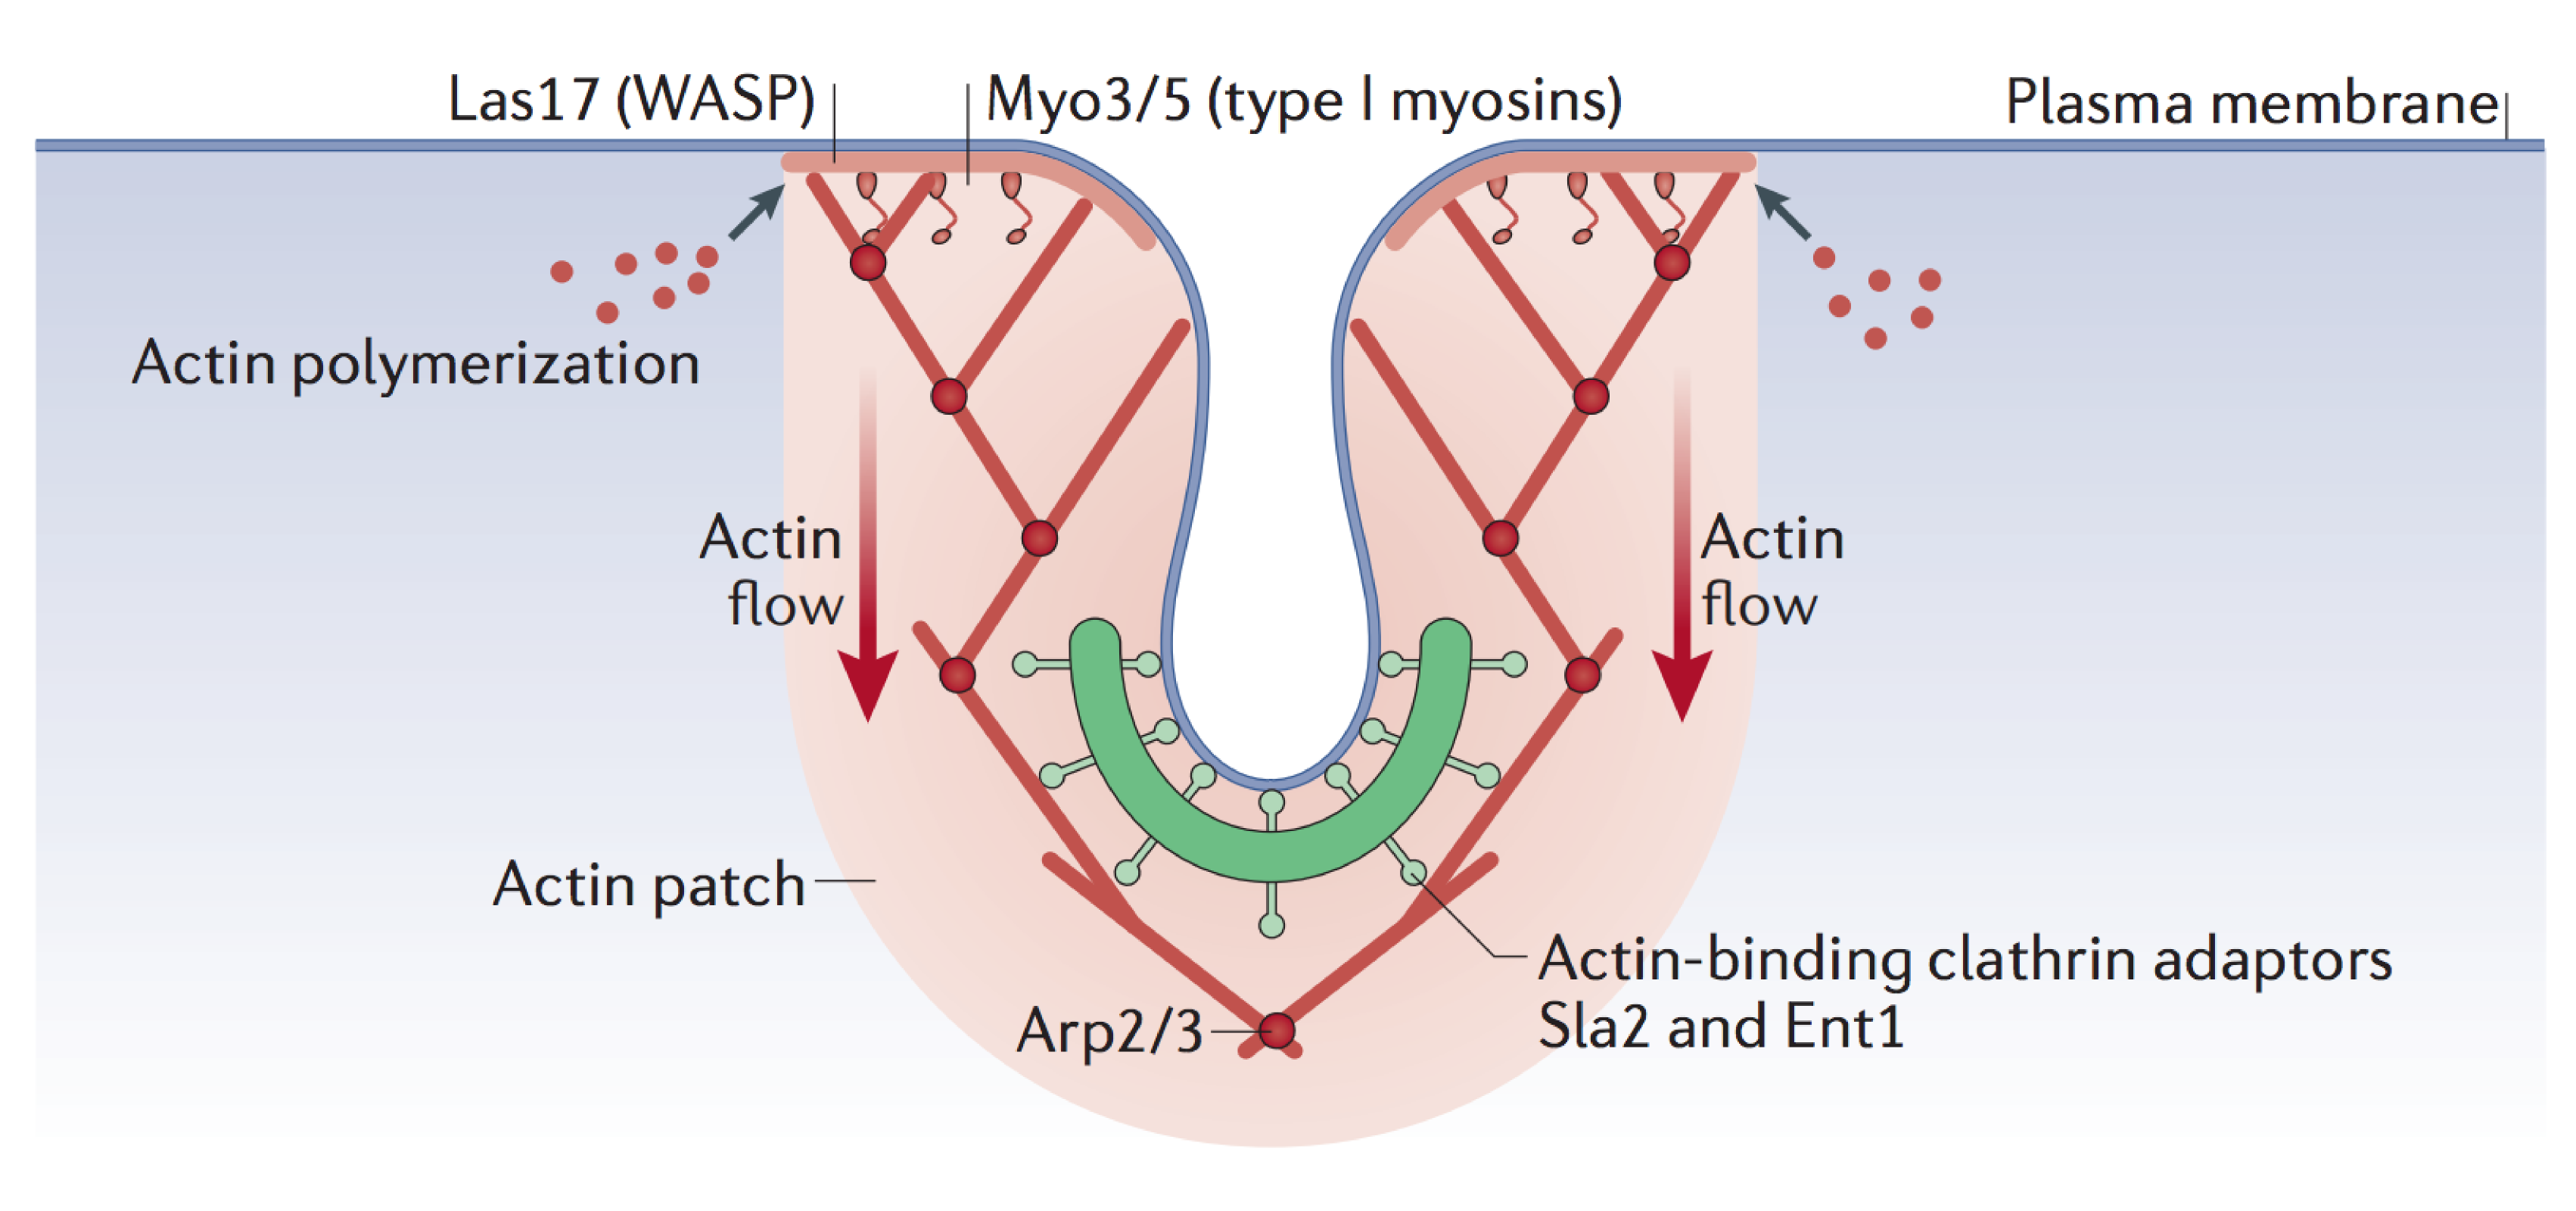
\includegraphics[scale=0.8]{figures/intro/actin_kaksonen}
			\end{figure}

			\subsubsection{Scission module}
		While the role of the yeast dynamin-like Vps1 is unclear, relatively few copies of the Rvs complex are recruited in a time window that spans only a few seconds, and membrane scission occurs when the invagination is about 140nm long, indicating tight regulation of this transition 30,34. Coat proteins and the actin network are rapidly disassembled by phosphorylation and dephosphorylation of the components.  What actually regulates scission in yeast is not yet determined (see \ref{yeast_scission}).


\begin{figure}[H]
	\centering
	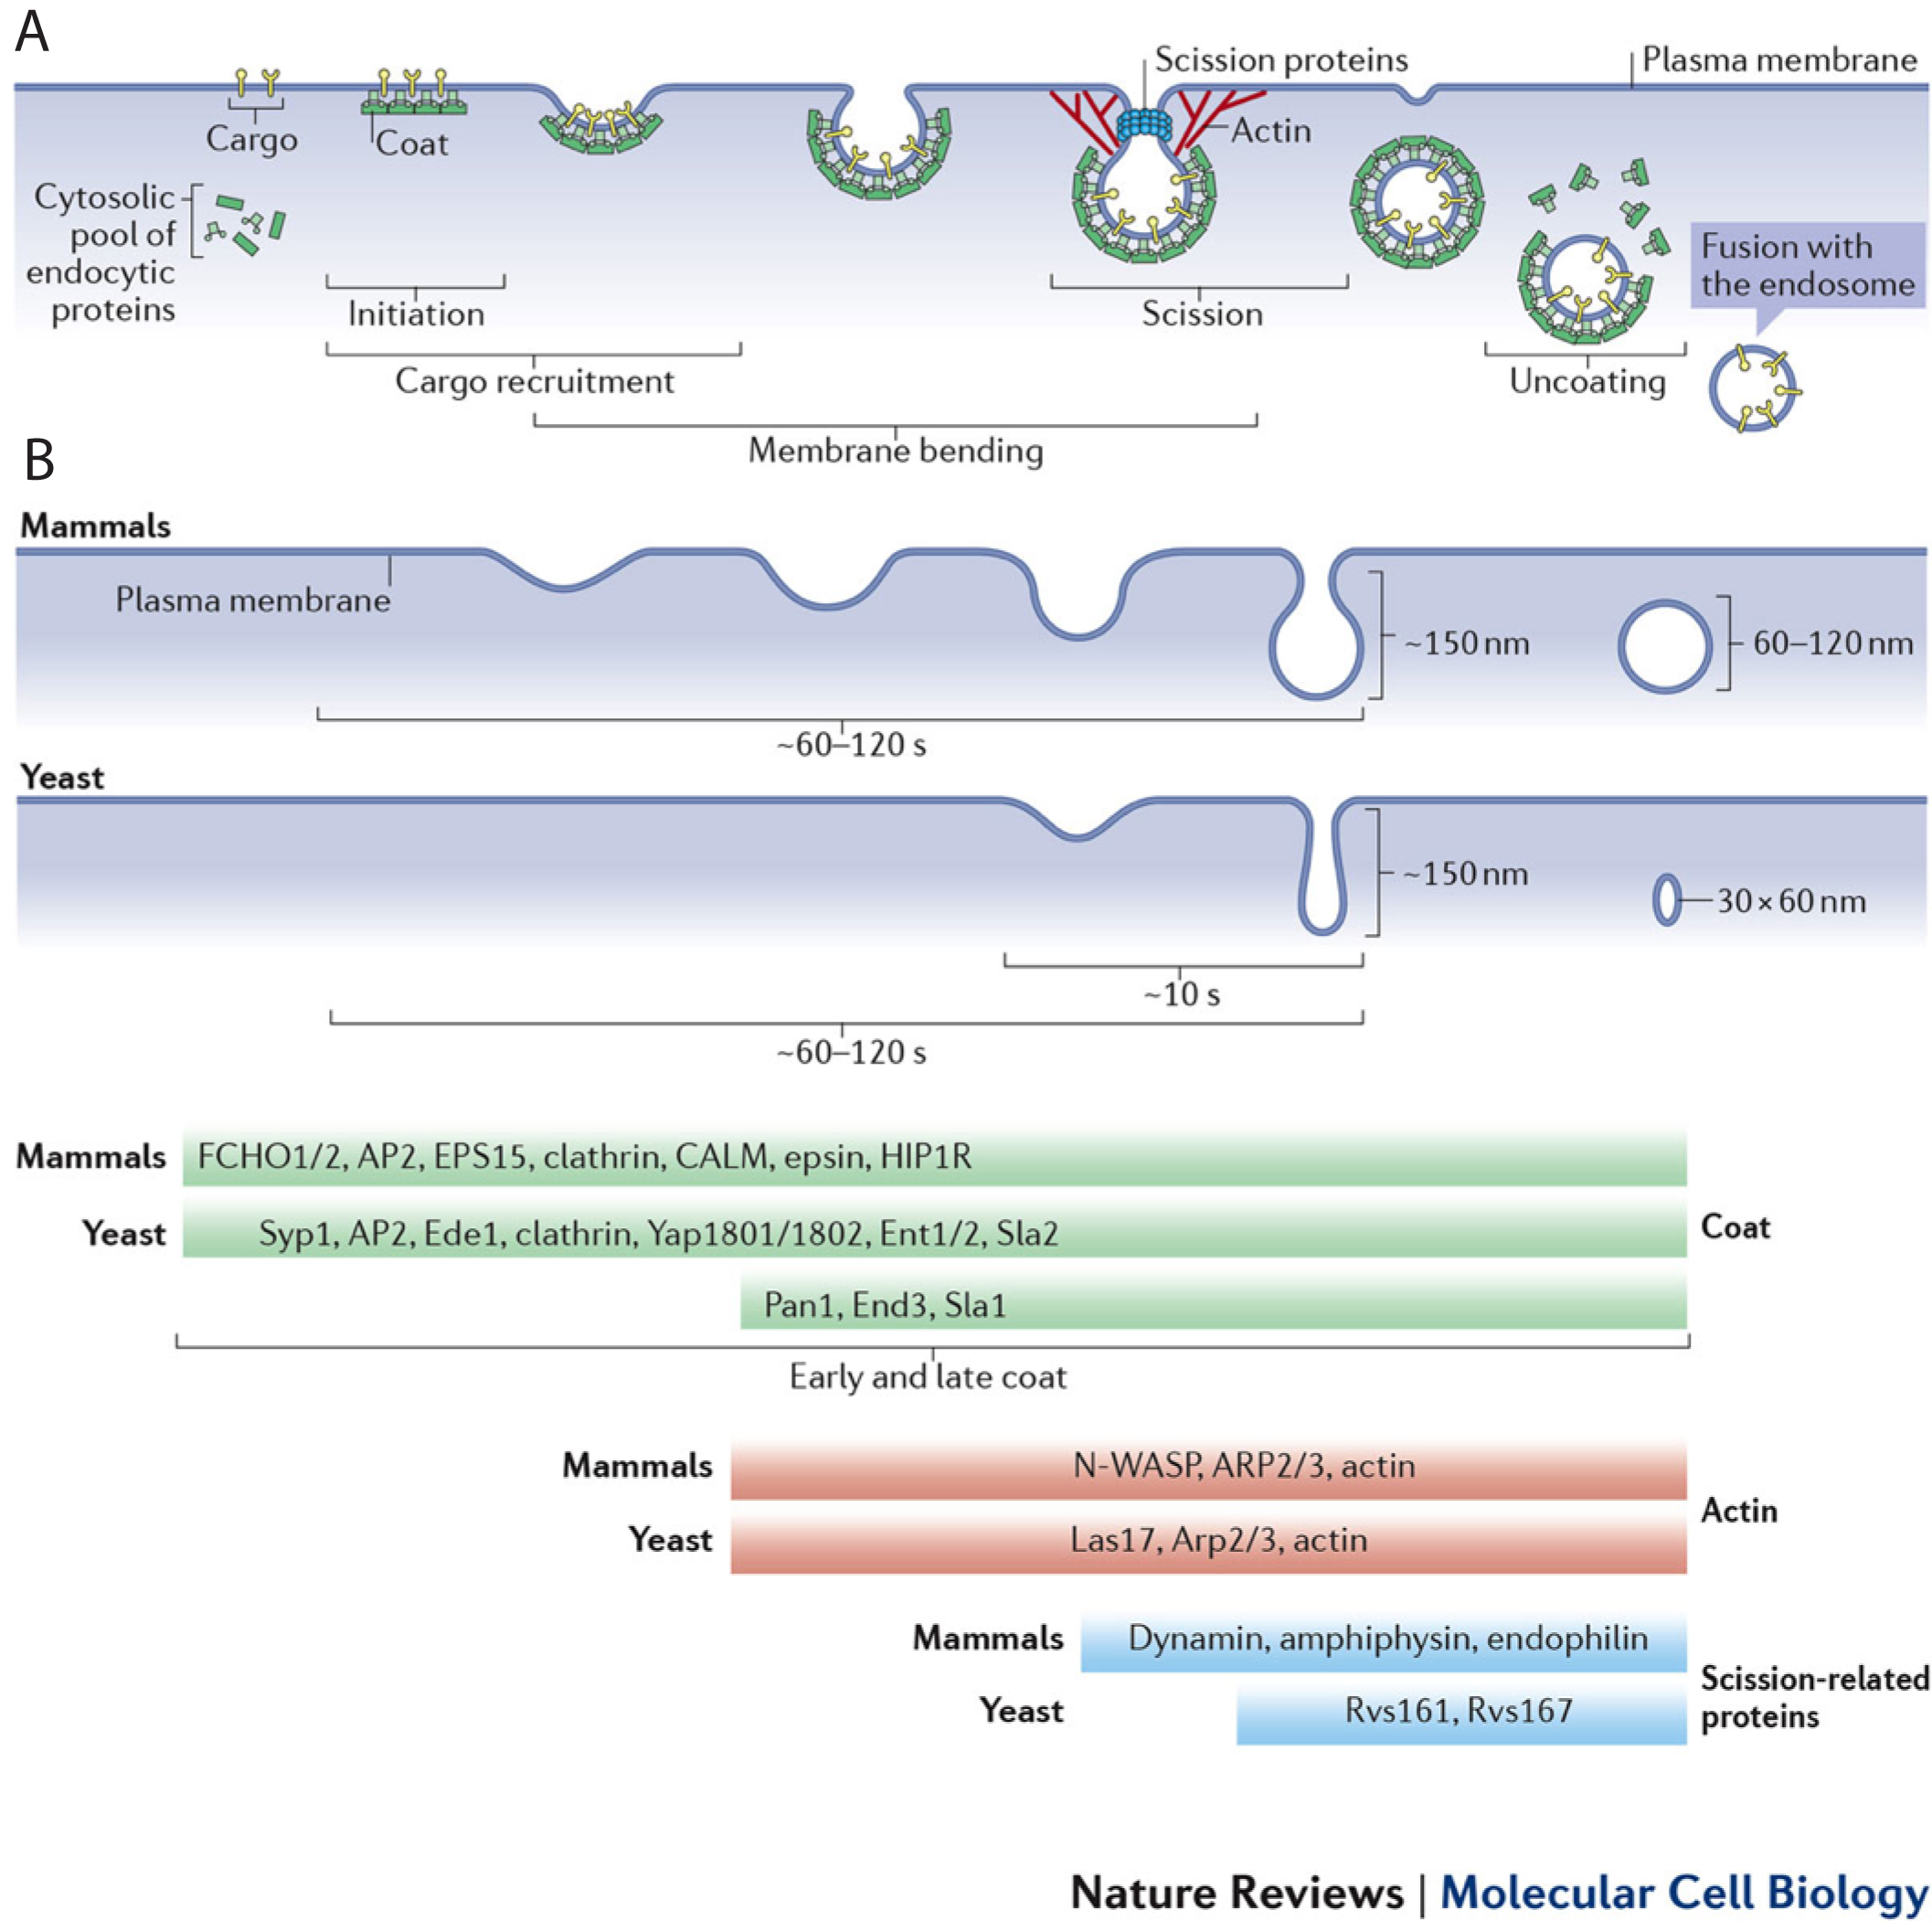
\includegraphics[scale=0.8]{figures/intro/Fig2_kaksonen}
\caption[Endocytic pathway in mammalian and yeast cells]
{A: Proteins involved in endocytosis are recruited from a cytoplasmic pool. Initiation of an endocytic event and cargo recruitment is followed by membrane bending. Membrane scission eventually forms a vesicle that releases its components, allowing it to be transported down the trafficking pathway. B: Membrane invagination in mammalian cells results in wider vesicles than in yeast cells. Proteins that are involved can be grouped based on their function in the endocytic pathway. Shown here are the main proteins involved, that are conserved between the two species. 
	\textit{Reprinted by permission from Springer Nature: Nature Reviews Molecular Cell Biology (Kaksonen and Roux, 2018), copyright (2018)}}
\end{figure}
		
\subsection{Membrane scission in mammalian cells}
		\subsubsection{Scission is dependent on dynamin} 
		In mammalian cells, membrane scission in endocytosis is primarily effected by the GTPase dynamin. Dynamin was discovered as a microtubule interacting protein 46, and since has been shown to have a pivotal role in membrane scission and fission at many different organelles across the cell. The importance of dynamin in endocytosis was demonstrated in a temperature sensitive mutant of the Drosophila shibire gene, which results in paralysis of flies at the non-permissive temperature. These flies fail to form synaptic vesicles 47–49. Shibire codes multiple isoforms of dynamin that are differentially expressed across the organism 50. Knock-down of dynamin isoforms results in initiation of clathrin-coated pits, but vesicle formation is disrupted, resulting in accumulation of a large number of long membrane tubes 51. 

		 
		\subsubsection{Dynamin is an oligomeric GTPase}
%		PIP\textsubscript{2}
		Dynamins consist of a GTPase domain, a stalk region, a bundle signalling element that acts as the linker between the GTPase domain and stalk, a PIP2-binding pleckstrin homology domain (PH) domain and a proline rich domain (PRD) that extends beyond the GTPase domain52. In-vitro, dynamin oligomerizes into helical structures with the PH domain apposed against the membrane, and the GTPase domain facing away from the membrane 53,54. Dynamin within the helical structure undergoes conformation changes upon GTP hydrolysis that constricts the helix as well as the membrane tube under it, collapsing the inner leaflet of the bilayer membrane into a hemi-fused state, resulting in membrane fission55. Disruption of its GTPase activity results in membrane tubes that accumulate dynamin, as well as the BAR domain proteins endophilin and amphiphysin56–58
		
%		\begin{figure}[H]
%			\centering
%			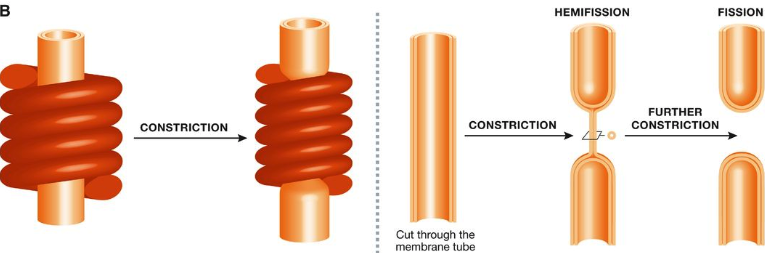
\includegraphics[scale=0.5]{figures/intro/dynamin_2}
%			\caption[Membrane fission by dynamin constriction]
%			{ Schematic of constriction by 
%				\texit{Reproduced from Antonny et al, under Creative Commons Cttribution Non-Commercial No Derivatives Licence CC BY-NC-ND}
%			\label{intro_dynamin_scission}}
%		\end{figure}


%(Adam et al., 2015) under creative commons licence \href{https://creativecommons.org/licenses/by/4.0/}{CC BY 4.0}}}

		\subsubsection{Dynamin interacts with BAR proteins to cause scission}
		Dynamin arrives at clathrin-coated pits via interaction with BAR proteins endophilin and amphiphysin51. BAR domain proteins form intrinsically curved protein dimers named for the conserved module contained in their founding members, metazoan BIN/ Amphiphysin and yeast proteins Rvs167, Rvs161. In addition to the BAR domain, most BAR proteins have additional motifs that mediate their interaction with membranes or other proteins: some BAR proteins have an N-terminal amphiphatic helix (N-helix) that is inserted into the membrane, phosophoinositide binding motifs like phox or pleckstrin homology (PH) domains direct BAR proteins to specific lipids within membranes, some BAR proteins have Src homology 3 (SH3) domains that mediate protein-protein interaction. These SH3 regions act as a scaffold for the proline-rich domains of dynamin 59. 


		\subsubsection{Dynamin and BAR proteins interact via PRD and SH3 regions }
		Dynamin’s PRD interacts with the SH3 domains of BAR proteins endophilin and amphiphysin59–62. Endophilin recruitment is reduced in the absence of dynamin, and appears to inhibit the GTPase action of dynamin60,62,63, while dynamin recruitment is decreased without endophilin. Amphiphysin levels are unchanged in absence of dynamin, while deletion of amphiphysin results in increased recruitment and prolonged lifetimes of dynamin and absence of membrane scission60. These results suggest a role for amphiphysin for disassembly of dynamin involving GTP hydrolysis, and a role for endophilin in dynamin assembly, although the mechanistic interplay between the two BAR proteins with dynamin is still debated, and the sequence of events is not clear63,64. Dynamin localization to localize to clathrin-coated pits is not dependent on BAR proteins, but both GTP hydrolysis and interaction with BAR proteins is necessary for efficient vesicle scission60,65.

\label{key}

	\subsection{Membrane scission in yeast} \label {yeast_scission}
		\subsubsection{Yeast dynamin-like proteins}
		In yeast, three dynamin-like large GTPases have been identified: Vps1, Dnm1, and Mgm1. Dnm1 and Mgm1 are involved in mitochondrial fission and fusion66. Vps1 is essential for vacuolar protein sorting67, is involved in fission and fusion of vacuoles68 and peroxisomes69, is required for regulation of golgi to endosomal trafficking70, and may arrive at early endocytic events71. None of the three yeast dynamins have the typical PH domain72,73 that in mammalian interacts with the lipid bilayer. Instead, an “InsertB” region likely performs the same function. Although yeast dynamins also do not have PRDs that could interact with the SH3 domains of yeast BAR proteins, Vps1 has been shown to interact with the clathrin and other endocytic proteins 71,74,75, though other work has failed to observe localization of Vps1 at endocytic sites41,74. The role of Vps1 in endocytosis is not clear, but it is a candidate for the role of the canonical dynamin in CME.


		\subsubsection{Yeast BAR domain proteins Rvs161/167 regulate scission timing}
		In yeast, the Amphiphysin/ Endophilin homologue is the heterodimeric complex Rvs161/16776 (Rvs), of which Rvs167 has an SH3 domain. Rvs arrives at endocytic sites in the last stage of the endocytosis, and disassembles rapidly at the time of membrane scission34. Deletion of Rvs results in failure of membrane scission in nearly 30\% of endocytic events26. Scission failure is identified by the movement inwards of the plasma membrane into the cytoplasm, followed by its retraction back towards the cell wall, indicating a failure to form vesicles. No mutation of known endocytic proteins exhibits this phenotype, while some mutations like that of the yeast Syndapin Bzz1 and Synaptojanin Inp52, in the background of rvsΔ, exacerbates the retraction phenotype41. This unique profile suggests that although Rvs is not necessary for scission, localization of the complex makes scission more efficient, and Rvs likely acts in concert with other proteins to effect this efficiency. 

		\subsubsection{What causes scission?}
		How Rvs may affect scission has not been determined. Since yeast dynamins do not have a PRD, there is likely no interaction with Rvs, so a mechanism that does not involve PRD-SH3 interactions like in mammalian cells is likely necessary. Yeast cells are under high turgor pressure that makes forces from actin polymerization necessary for invagination77,78. There is therefore likely to be some interplay between scission-stage proteins and the actin network that could modulate the final shape transitions. 

		
			\subparagraph{Proposed scission mechanisms}
			\mbox{}\\
			Several scission models have been presented in the literature so far. Yeast dynamin is the obvious solution to membrane scission. Although none of the three dynamin-like proteins has a proline-rich domain, Vps1 has been suggested to play a role in endocytosis71. \textit{vps1\textDelta} \textit{rvs167\textDelta}  double mutant has been shown to increase membrane retraction rates after invagination79, an indication of scission failure. Another hypothesis has proposed that lipid hydrolysis by yeast synaptojanin-like proteins can cause vesicle scission80. Synaptojanins dephosphorylate PIP2, a lipid subtype enriched at endocytic sites. In this model, Rvs would form a scaffold on the membrane tube, protecting the underlying PIP2 and causing a boundary between BAR-protected PIP2 at the tube and hydrolyzed PIP2 at the bud tip. This lipid boundary produces a line tension at the interphase that could generate enough force to pinch off a vesicle. 
			
			\vspace{5mm}
			\textit{In-vitro} experiments have proposed protein friction as a mechanism by which membrane scission could occur81. In this model, a BAR domain scaffold exerts a frictional force on a membrane that is pulled under it. Such a friction-dependent membrane scission model would predict that if more BAR proteins are added to the membrane, frictional force would increase, and scission should occur at shorter invagination lengths. In-vivo, this pulling force is generated by actin polymerization. 


			\vspace{5mm}
			Recently, steric pressure exerted on the membrane by disordered protein domains that typically follow the BAR region has been proposed as a mechanism for scission82. In these experiments, the amphiphysin BAR domain is able to drive scission, but scission efficiency increases three to four-fold because of the disordered protein domains, and these domains do not need to have any specific biochemical properties: they can be replaced by any other disordered protein region. It has also been proposed that BAR domain scaffold membrane tubes and stabilize them, preventing scission83,84. For a more detailed discussion on these models, see /ref{results}


			\vspace{5mm}
			Many of these theories are contradictory, based on in-vitro data, using mammalian BAR proteins, at concentrations of protein orders of magnitude higher than physiological levels, and without the context of interaction partners, relevant membrane tension, native lipid composition and intra-cellular turgor pressure: a mechanism for membrane scission in yeast is yet to be determined. 


		
\section{BAR domain proteins}
	
The BAR protein superfamily have a highly conserved BAR domain structure across eukaryotes and are involved in a range of cellular processes including endocytosis, actin organization, cell polarity, transcription and tumor suppression85,86. 
Of the mammalian isoforms of the founding members, Bin1 (Amphiphysin II) and Bin3 are ubiquitously expressed, while Amphiphysin I is expressed only in neurons. The conserved portion of these proteins, as well as of Rvs167 and Rvs161, is an N-terminal region that forms the BAR domain. This domain typically forms dimers with other BAR domains, and have an intrinsic curvature defined by the dimerization angle. This curvature categorizes BAR proteins to classical BAR, Fer–Cip4-homology-BAR (F-BAR, shallow curvature), and I-BAR (inverted curvature). Membrane-binding is mediated by cationic clusters that bind via non-specific electrostatic interactions to anionic lipids like phosphatidyl serine (PS) or phosphatidylinositol (4,5)-bisphosphate (PtdIns(4,5)P2, henceforth PIP\textsubscript{2}).

\vspace{2mm}

\begin{figure}[H]
	\centering
	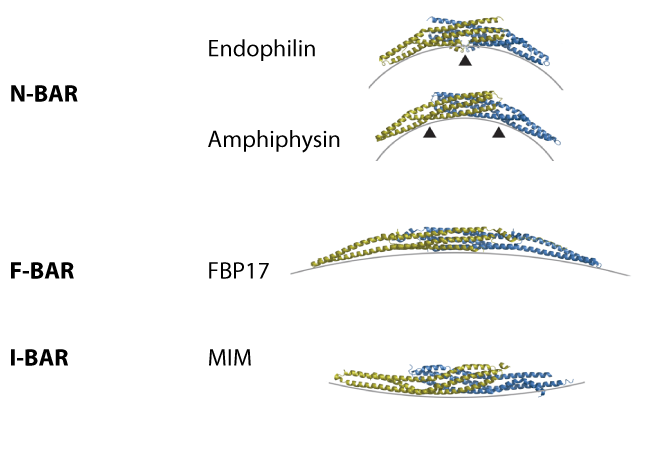
\includegraphics[scale=0.6]{figures/intro/BAR_structures}
		\caption[Structures of BAR domain dimers]{Domain structures from different families of BAR proteins. One monomer is depicted in yellow, the other in blue. Arrow heads indicate positions on the BAR domain that are inserted hydrophobically into the membrane. \textit{Adapted with persmission from John Wiley \& Sons, Inc.: The EMBO Journal (Qualmann, Koch, and Kessels, 2011), copyright (2011)}
		\label{bar_structures}}
\end{figure}

\newpage
\vspace{5mm}
BAR dimers are able to oligomerize and scaffold large areas of membrane. These scaffolds can tubulate and generate curvature across membrane regions much larger than the dimensions of a BAR dimer62,87. BAR scaffolds can also bind membranes in a curvature-dependent manner. Correlation between the membrane shapes that they bind in-vivo and their intrinsic curvature has been shown for many BAR proteins: they may induce, stabilize, or generate specific curvature within cells. 

		
\begin{figure}[H]
	\centering
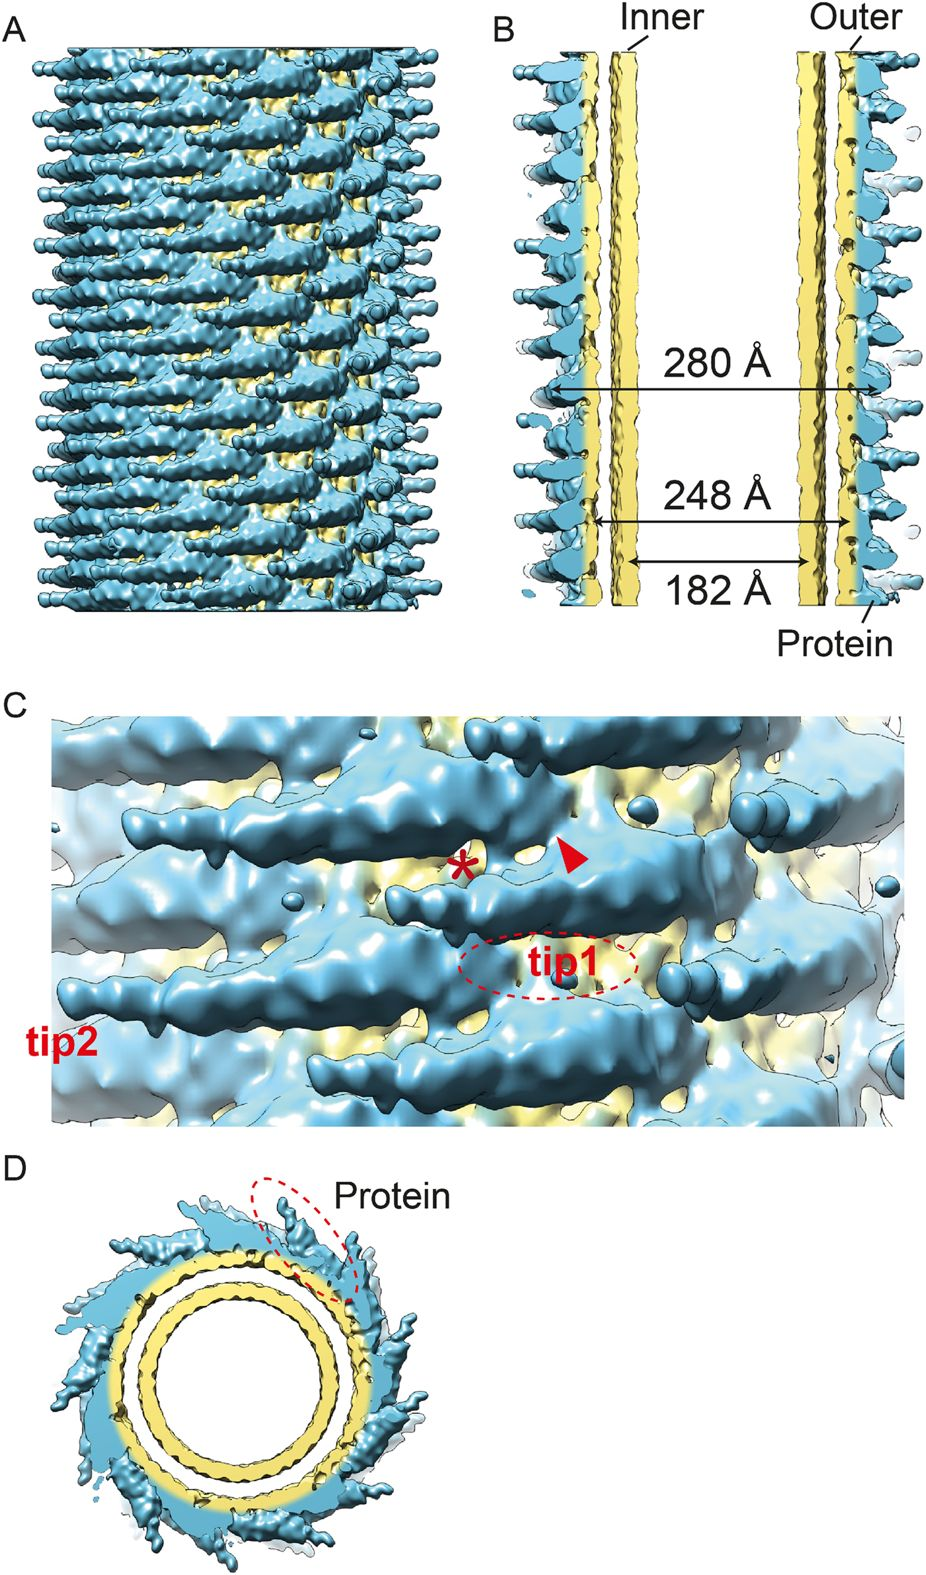
\includegraphics[scale=0.4]{figures/intro/BAR_scaffold}
\caption[BAR domain scaffolds]
{A: 3D reconstruction of amphiphysin-mediated tube from cryo-EM. Protein densities in blue,  lipid densities in yellow. B: Inner and outer leaflet of membrane is indicated. Numbers correspond to total diameter, and diameter of inner and outer membrane tubes. \textit{Figure reprinted from (Adam et al., 2015) under creative commons licence \href{https://creativecommons.org/licenses/by/4.0/}{CC BY 4.0}}}
	\end{figure}



	\subsection{NBAR proteins and membrane shapes}	
	Classical BAR domain proteins form a crescent-shaped structure. Some of them have an N-terminal amphiphatic helix (N-helix), forming a subclass of classical BAR called NBAR domains. The two significant endocytic BAR proteins, Endophilins and Amphiphysins, are NBAR proteins. The 35-40 residue N-helix acts as an amphiphatic wedge that is unstructured until it is inserted into the upper leaflet of a membrane bilayer 87. The insertion causes displacement of lipids, resulting in bending of the membrane, indicating that N-helix insertion into a membrane bilayer could favor membrane scission both energetically and kinetically 84,88. BAR domains lacking this helix are not able to efficiently tubulate vesicles89. The N-helix also increases efficiency of binding to liposomes62 in a curvature sensitive manner, and confers salt sensitivity89. 


	\vspace{5mm}
	High resolution structural data has shown that NBAR proteins can hold form helical scaffolds on tubular membranes 87,90,91. An energetically favorable arrangement of BAR domains consist of dimers parallel to each other, apposed to the membrane, supporting membrane tubulation and preventing scission by stabilizing the membrane tube84. Hybrid N-helix and BAR scaffolds can therefore allow coexistence of both vesicles and tubules, with preference for one or the other depending on the ratio between number of N-helices that favor vesiculation, and BAR generated scaffold stability 84. 


	\vspace{5mm}
	Both BAR proteins implicated in CME , Amphiphysin and Endophilin are shown to tubulate membranes in-vitro87,89,91 and form a helical scaffold. The tubulation diameter resembles the diameter of the proteins themselves, and involve lateral interactions of the neighboring BAR domains92. Both BAR domains are able to form mixed helices in the presence of dynamin62,93. 


	\subsection{NBAR protein in endocytosis: Amphiphysin }		
%		\subsubsection{Classical BAR domains : Amphiphysin}
	Two mammalian isoforms of Amphiphysins (Amph) are found. AmphI is enriched in neurons in mammals, while AmphII (Bin1) is expressed in other tissue types, with one isoform enriched in muscle T-tubule junctions94. The only Amphiphysin (d-Amph) in flies is expressed in various tissues, and enriched at muscle T-tubule junctions in flies. The d-Amph dimer forms a coiled coil, with each BAR domain made of three long, kinked alpha-helices87. In-vitro, liposome tubulation activity of Amphiphysin is concentration dependent, at very high concentrations, it is also able to sever tubular membrane to form vesicles87. 


	\vspace{5mm}
	Amph I and II both have BAR domains, a proline rich region, and C-terminal SH3 domain.
Amphiphysin I, but likely not II binds Clathrin and its adaptors95 and can polymerize clathrin into invaginated lattices in a BAR domain dependent manner87, while both bind dynamin, and the lipid phosphatase Synaptojanin61.


	\subsection{NBAR protein in endocytosis: Endophilin }	
%		\subsubsection{Classical BAR domains : Endophilin}
	Endophilins A1-A3 (EndoA) were discovered as SH3 domain containing proteins 96 that co-localized with dynamin, and interacted with Synaptojanin58 and amphiphysin97: all already identified as important regulators of synaptic vesicle recycling by endocytosis. A second mammalian protein was later discovered as related, and then termed EndophilinB (EndoB). Other sequenced eukaryotes have a single isoform of EndoA and B.

	\vspace{5mm}
	EndoA1-3 isoforms are found in neurons, ubiquitously, and enriched in the brain and testes respectively. All three are found at presynaptic membranes. Crystal structure of EndoA1 shows essentially the same structure as that of amphiphysin, with an additional amphiphatic helix similar to the N-helix, located at the centre of the crescent-shaped dimer89,98. This helix is thought to insert into the membrane in the same way as the N- helix, potentially inducing faster tubulation of membranes. EndoA1 and 2 may interact with calcium channels at synapses, and may be involved in lipid modification99,100, suggesting different roles for the two BAR domain proteins in membrane interaction. Endophilin interacts with dynamin, NWASP and Synaptojanin proteins via its SH3 domain61,63,101



	\subsection{NBAR protein in yeast endocytosis: the Rvs complex}		
	RVS167 and RVS161 (reduced viability upon starvation) genes were discovered in a screen that tested for survival under starvation conditions102. Rvs167 and Rvs161 are both NBAR domain proteins that thought to form obligate heterodimeric complexes (Rvs) in-vivo103,104. Although there is evidence of heterodimerization: loss of one destabilizes the other, deletion phenotypes of Rvs167 is the same as that of Rvs161, and FCCS measurements indicate that they dimerize 26,103,105, it has also been reported that Rvs161 has some functions that do not match that of Rvs167. Rvs161 for instance, interacts with Fus2 in cell-cell fusion, while Rvs167 does not106. It is consistent however, that at endocytic sites they function together as heterodimers. 

		
	\vspace{5mm}
	Rvs161 and Rvs167 are similar in structure at the N-terminus, both contain NBAR domains that are 42\% similar, and although share 21\% identity, are not interchangeable107. In addition to the BAR domain, Rvs167 has a Glycine-Proline-Alanine rich (GPA) region and a C-terminal SH3 region. The GPA region is thought to act as a linker with no known other function, while loss of the SH3 domain affects budding pattern and actin morphology. Most Rvs deletion phenotypes can however, be recapitulated by expression of the BAR domain alone104, suggesting that the BAR domains are the main functional unit of the complex 

	\vspace{5mm}
	Deletion of the genes show abnormal actin morphology, confer salt sensitivity, as well as amino-acid and lipid sensitivity, and have abnormal budding pattern103,108–110. Homology modelling has shown that the BAR domain of Rvs167 is similar to Amphiphysin and Endophilin, and is therefore also likely to function similarly to the mammalian homologues. In keeping with this theory, Rvs has been shown to tubulate liposomes in-vitro111. 

		
	\vspace{5mm}
	Averaged centroid tracking of the Rvs complex has shown that Rvs arrives in the scission stage of endocytosis. When maximum number of Rvs is recruited, that is, at peak fluorescent intensity, the centroid jumps inwards, concomitant with a sharp decay in fluorescent intensity. This behavior is unique among endocytic proteins, and since similarity in structure with Amphiphysin/ Endophilin BAR domains is expected, has led to the proposition that Rvs may also form a helical scaffold on the membrane tube, whose sudden disassembly either leads to or is caused by membrane scission. The sharp movement into the cytoplasm of the Rvs centroid is then caused by the disassembly of the scaffold, and a jump in the centroid position to the remaining Rvs on the base of the newly formed vesicle34. How Rvs is recruited to endocytic sites, and the cause of the scaffold disassembly are not known, and are the major questions addressed in this work.

\vspace{2mm}
\begin{figure}[H]
	\centering
	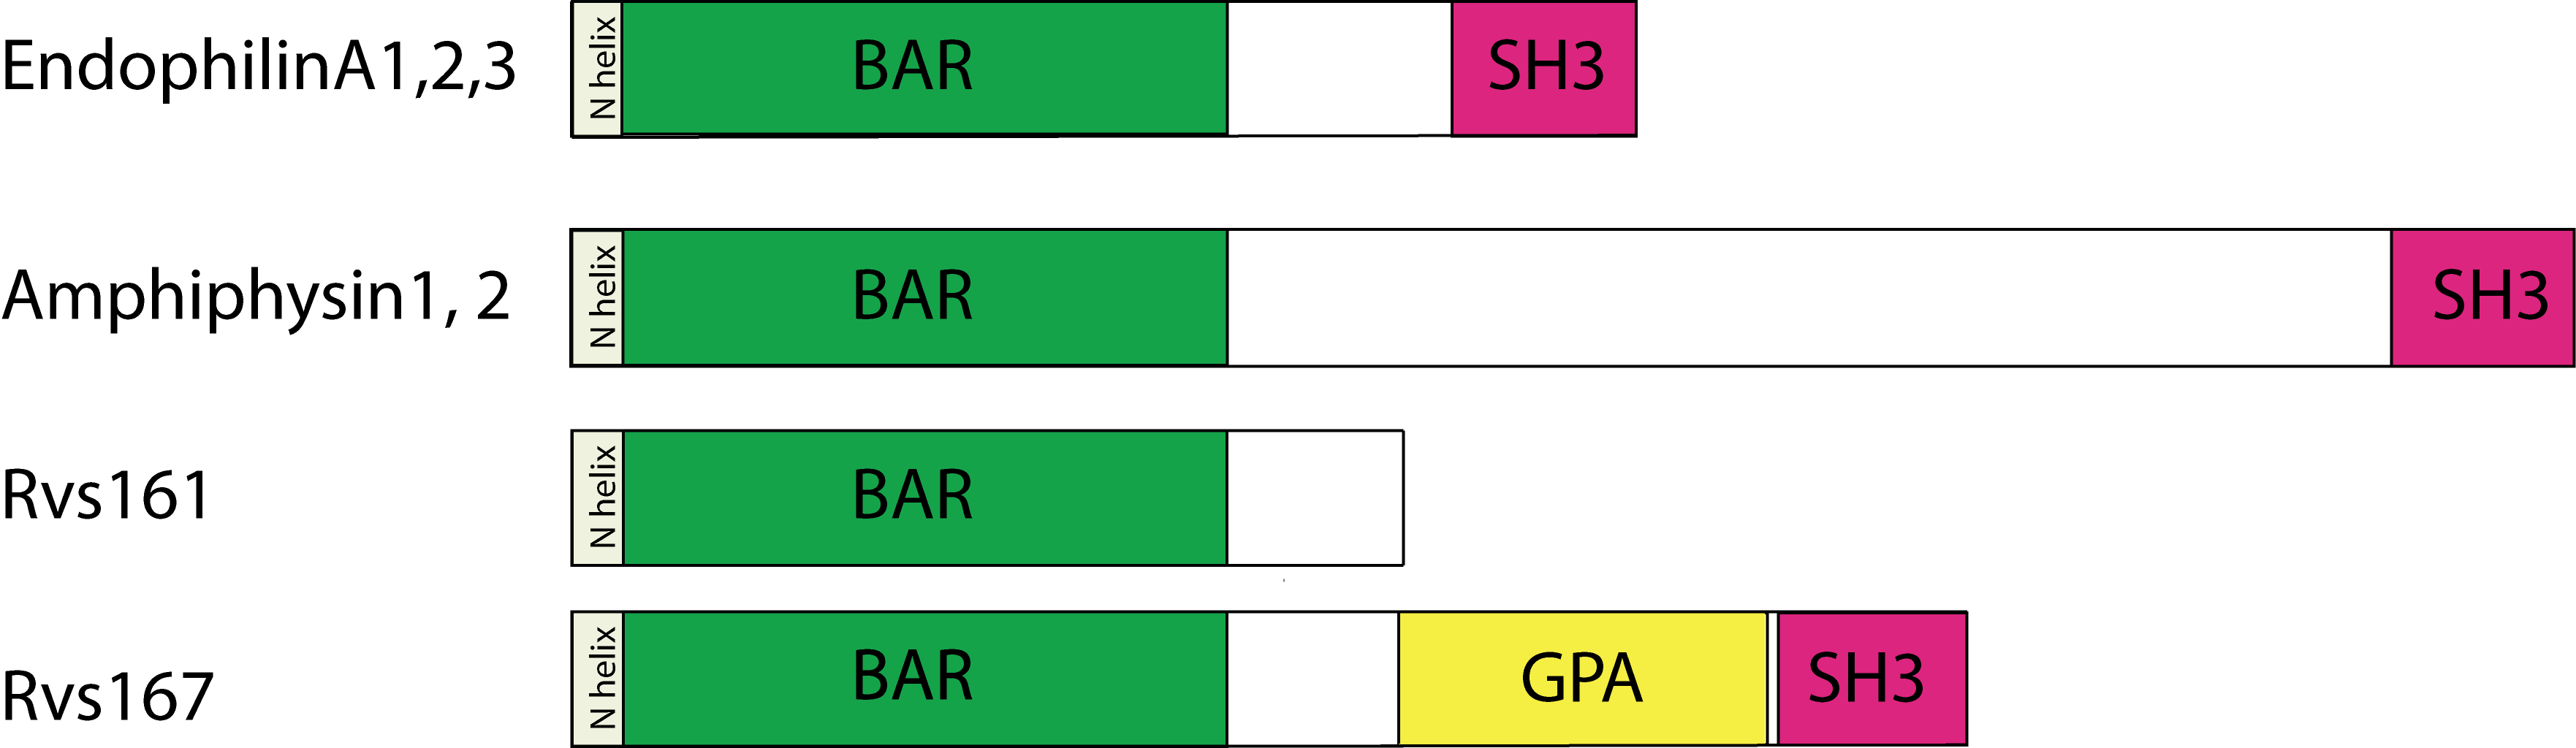
\includegraphics[scale=0.4]{figures/intro/BARdomainstruc2}
\end{figure}
		

%\begin{itemize}
%	\item Is localization microscopy suitable to study endocytosis in budding yeast?
%\end{itemize}
